% Part: biographies 
% Chapter: alfred-tarski 
% Section: biography
\documentclass[../../../include/open-logic-section]{subfiles}

\begin{document}

\olfileid{bio}{aft}{bio} 
\olsection{Biography}

\begin{figure}[h!] 
\centering
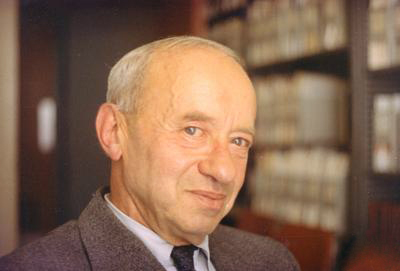
\includegraphics[scale=0.5]{alfredtarski.jpeg} 
\caption{Alfred Tarski. Photo Credit: The Oberwolfach photo collection.} 
\end{figure}

Alfred Tarski was born on January 14, 1901 in Warsaw, Poland (then part
of the Russian Empire). Although a rival of G\"{o}del in terms of his affect on the 
landscape of logic, his physical presence held no rival. Often described as 
"Napoleonic," Tarski was boistrous, talkative, and intense. His energy was often
reflected in his lectures - he once set  fire to a wastebasket while disposing of a
cigarette during a lecture, and was forbidden from lecturing in that building again
\citep[2]{feferman2004}. 

Tarski had a thirst for knowledge from a young age. Although later in life he would
tell students that he studied logic because it was the only class in which he got a B,
his high school records show that he got A's across the board - even in logic 
\citep[18]{feferman2004}. He studied at the University of Warsaw from 1918 to 1924.
Although intending to study biology, he became interested in mathematics, philosophy
and  logic, as the university introduced the Warsaw School of Logic and Philosophy
\cite[30]{feferman2004}. He earned his doctorate in 1924 under the supervision of 
Stanisław Le\"{s}niewski.

Before emigrating to the United States in 1939, Tarski completed some of his most
 important works while working as a secondary school teacher in Warsaw. His work
 on logical consequence and logical truth were written during this time. In 1939, Tarski
 was visiting the United States for a lecture tour, and because of his Jewish heritage,
 did not return before the end of the war. His wife and children remained in Poland
 until the war ended, and were able to emigrate to the United States as well. During 
 his time in the United States, Tarski taught at Harvard, the College of the City of New
 York, and the Institute for Advanced Study. He was also a founder of the multidisciplinary
 program in logic and the methodology of science at the Univeristy of California, Berkeley.
 Tarski passed away in 1983 at the age of 82.


\end{document}